\section{Introducción}

\begin{frame}{Automatas Celulares}
    \begin{block}{Son arreglos regulares de celdas individuales de la misma clase.}
        Caracteristicas:
        \begin{itemize}
            \item Finitos estados y discretos.
            \item Estados: Actualizan simultáneamente.
            \item Reglas de actualización determinísticas y uniformes.
            \item Solo se considera un vecindario local.
        \end{itemize}
    \end{block}

    \begin{multicols}{2}
        {Estados: $a_{i}^{(t)}$ $\rightarrow$ Celda $i$ en tiempo $t$}

        {Regla de evolución: $a_{i}^{(t)} = f \left[ \sum_{j=-r}^{j=r}  \alpha_{j} a_{i+j}^{(t-1)} \right]$}
    \end{multicols}

\end{frame}

\begin{frame}{Game of Life}

\end{frame}

\begin{frame}{Vecindario}
    \begin{block}{Von Neumann:}
        \begin{multicols}{2}

            $N_{i,j}^{vN}:=\{(k,l) \in L\ |\ |k-i|+ |l - j| \leq r\}$

            \begin{figure}[H]
                \centering
                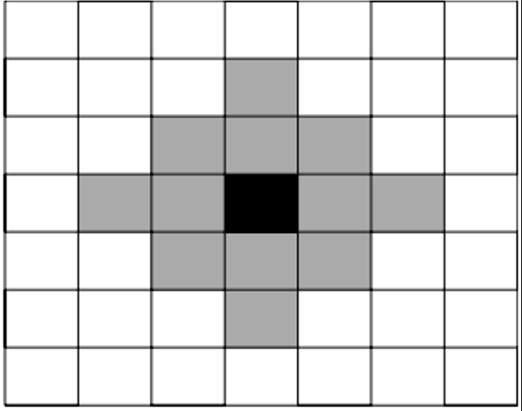
\includegraphics[width=0.3\linewidth]{pic/01-intro/vn}
            \end{figure}

        \end{multicols}
    \end{block}
    \begin{block}{Moore:}
        \begin{multicols}{2}
            $N_{i,j}^{M}:=\{(k,l) \in L\ |\ |k-i|\leq r\ \wedge \ |l - j| \leq r \}$

            \begin{figure}[H]
                \centering
                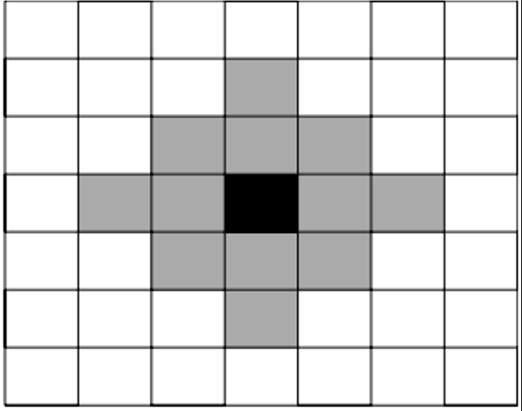
\includegraphics[width=0.3\linewidth]{pic/01-intro/moore}
            \end{figure}
        \end{multicols}
    \end{block}
\end{frame}

